  \chapter{Stimulated Raman Adiabatic Passage in Optical Lattices}
\index{Stimulated Raman Adiabatic Passage in Optical Lattices%
@\emph{Stimulated Raman Adiabatic Passage in Optical Lattices}}%
\label{chapter-optical_lattice}
\section{\label{sec:1} Introduction}
As we have seen for the double well case in chapter~\ref{chapter-dblwell}, avoided crossings of eigenvalue curves are an important feature of quantum systems with non-integrable classical counterparts. This was demonstrated theoretically by Von Neumann and Wigner as part of seminal work~\cite{von-Neumann:Wigner}. This phenomenon allows for many interesting phenomena related to chaos. In particular, the adiabatic exchange of character provides a mechanism by which the underlying classical chaos affects the quantum dynamics~\cite{na-reichl:pbox}~\cite{mypaper}. Their existence is responsible for the well-known phenomenon of 'quantum chaos' in the spectral statistics of the system~\cite{reichl}. In this chapter, we look at coherently controlled excitations of atoms trapped in an optical lattice via the same STIRAP technique used for the double well system in chapter~\ref{chapter-dblwell}. 

An optical lattice is a periodic potential formed by the AC Stark shift seen by atoms when they interact with interfering laser beams. The way that this potential is generated follows from the theory of light-atom interactions, and is shown in section~\ref{chapter-intro:section:lightatom}, and detailed specifically for the optical lattice in the next section. While optical lattice systems have been of great interest in experimental physics (see, for instance,~\cite{oplattice:oldexpt} and~\cite{oplattice:oldexpt2}) and theoretical physics~\cite{oplattice:oldtheory}~\cite{oplattice:oldtheory2} for some time, it was in 1992 when Graham, Schlautmann and Zoller proposed that dynamic localization of the type being discussed in this dissertation is achievable~\cite{graham}. Since then, such systems have sparked considerable experimental and theoretical interest.  The properties of ultracold atoms in optical lattices can be used to precisely control many-body systems and  function as analog quantum computers, allowing for exploration of physical regimes inaccessible in regular condensed-matter systems. This led to the discovery of groundbreaking physics in these systems, such as the famous superfluid-Mott insulator transition by Jaksch and Zoller in 1998~\cite{sfmi:theory} (later seen experimentally by Grenier, Mandel,  Esslinger, Hansch and Bloch~\cite{sfmi:expt}). The dynamics of chaos in these systems has also been the subject of attention in recent years~\cite{graham}, including chaos as reported by Graham, Schlautmann and Zoller themselves. The dynamics and the influence of chaos in such dynamics is an important factor in the manipulation of such systems~\cite{raizen:oplattice}, such as the coherent acceleration of atoms from stationary to mobile states~\cite{holder:reichl:2res}. More recently (2009), number squeezing and subpoissonian distribution of atoms in each site in an optical lattice have been reported by Itah et al that is similar to the atom culling considered for the double well in chapter~\ref{chapter-dblwell}~\cite{technion:oplattice-culling}.

The optical lattice system that we will be investigating is a two-parameter system of the harmonically driven pendulum which has been implemented in a number of experimental studies~\cite{steck}~\cite{luter:reichl:3res} through ultracold atom optical systems. In the following sections, we will study the properties of avoided crossings for the driven pendulum with the use of Floquet theory as we did for the double well system in chapter~\ref{chapter-dblwell}. We will facilitate a time dependent 'radiation pulse' by the use of multiple resonances from mobile lattices that share the same period as the stationary lattice. Avoided crossings in the Floquet states can be associated with real transitions of the undriven eigenstates, and is an indication of the influence of deterministic chaos in the quantum dynamics of this system.

\section{\label{sec:2}The Basic Model}
We saw in chapter~\ref{chapter-intro} section~\ref{chapter-intro:section:lightatom} that an atom, confined in one dimension, it's dynamics described by a single outermost electron, and subjected to a laser field far detuned from it's internal atomic resonances, can be described by a 'Reduced Atom' Hamiltonian.
\begin{equation}
H(x)=\frac{p^2}{2m}+\frac{\hbar^2 \Omega^2(x)}{4\Delta}.
\label{eq:redatom:chapter-oplattice}
\end{equation}
Here, $\Omega(x)$ is the Rabi frequency defined by Eqn~\ref{eq:rabifreq:chapter-intro}. 

Now, if the electric field is produced by $M$ lasers, all polarized in the $z$-direction, such that the $j^{th}$ laser is projected with a frequency that is slightly deviated by a factor $\left[ \frac{\delta \omega_j}{2},\frac{ \delta k_j}{2} \right]$  from a fixed $\left[ \omega,k \right]$~\footnote{The derivation shown here is based on the noninteracting case shown in~\cite{holder:thesis}}, we have
\begin{equation}
E_z(x,t) = \sum^{M}_{j=1} E^{j}_0 \exp{\left[ i \left\{ \left( k+\frac{\delta k_j}{2} \right)x + \sigma_j \left(\omega+\frac{\delta \omega_j}{2} \right)t \right\} \right]}.
\label{eq:lasers:chapter-oplattice}
\end{equation}
Here, $\sigma_j=\pm 1$ decides the direction of propagation in the $x$ direction, and $\delta \omega_j=c\delta k_j$. If $M=2$, and the two lasers are counterpropagating in the $x$ direction with the same amplitude and wavelength, Eqn~\ref{eq:lasers:chapter-oplattice} gives us $E^{Re}_z(x,t)=E_\kappa \left[ \cos{\left(kx-\omega t \right)} +\cos{\left(kx+ \omega t \right)} \right]=E_\kappa(x) \cos{\omega t}$, where $E_\kappa(x)=E_\kappa \cos{kx}$. Plugging $E_\kappa(x)$ into Eqn~\ref{eq:rabifreq:chapter-intro} and then into Eqn~\ref{eq:redatom:chapter-oplattice} gives us the Hamiltonian for this system viz.
\begin{equation}
H(x)=\frac{p^2}{2m}+\kappa \cos{\left( 2 kx \right)},
\label{eq:standingwave:chapter-oplattice}
\end{equation}
where $\kappa=\frac{\hbar^2 E^2_\kappa}{4\Delta}$. This system is a standing wave optical lattice of frequency $2 k$. Also, this system is basically just the quantum pendulum, and it's eigensystem consists of Mathieu functions and their characteristics for the energy eigenvalues~\cite{reichl}~\cite{abramowitz:stegun}. 

Now, if the two counter-propagating lasers are slightly off in their frequencies by a factor $\pm  ({\delta \omega}/2,{\delta k}/2)$, we then get a traveling electric field
\begin{multline}
E_z(x,t) =  E_\lambda  \exp{ \left[ i \left\{ \left( k-\frac{\delta k}{2} \right)x +  \left(\omega-\frac{\delta \omega}{2} \right)t \right\} \right] } \\
  +  E_\lambda \exp{\left[ i \left\{ \left( k+\frac{\delta k}{2} \right)x -  \left(\omega+\frac{\delta \omega}{2} \right)t \right\} \right]}.
\end{multline}
Taking the square of the above and neglecting the rapidly oscillating terms, we get 
\begin{equation}
E^2_z(x,t) = E^2_\lambda e^{i\left(2kx - \delta \omega t \right)}.
\end{equation}
Plugging the real part into Eqn~\ref{eq:rabifreq:chapter-intro} and then into Eqn~\ref{eq:redatom:chapter-oplattice} gives us an optical lattice traveling with speed $\delta \omega$ viz
\begin{equation}
H(x)=\frac{p^2}{2m} + \lambda \cos{\left( 2kx-\delta \omega t \right)},
\end{equation}
where $\lambda=\frac{\hbar^2 E^2_\lambda}{4\Delta}$ for the amplitude of this laser. Combining this with the standing wave configuration of lasers in Eqn~\ref{eq:standingwave:chapter-oplattice} gives us a time periodic two-resonance Hamiltonian
\begin{equation}
H_{2res}(x)=\frac{p^2}{2m} +\kappa \cos{\left( 2 kx \right)}+ \lambda \cos{\left(2kx-\delta \omega t\right)}.
\label{eq:twores:chapter-oplattice}
\end{equation}
Duplicating the same pair of lasers, but moving in the opposite direction, produces the time periodic three-resonance Hamiltonian. 
\begin{equation}
H_{3res}(x)=\frac{p^2}{2m} +\kappa \cos{\left( 2 kx \right)}+ \lambda \cos{\left( 2kx \right)}\cos{\delta \omega t}.
\label{eq:threeres:chapter-oplattice}
\end{equation}
If we subjected this system to a similar pair of frequency-offset lasers, we would get a five-resonance Hamiltonian
\begin{equation}
H_{5res}(x)=\frac{p^2}{2m} +\kappa \cos{\left( 2 kx\right) }+ \lambda \cos{\left( 2kx \right)} \cos{\delta \omega t}+\lambda' \cos{\left( 2kx \right)} \cos{\delta \omega ' t}
\label{eq:fiveres:chapter-oplattice}
\end{equation}
In the limit $\lambda, \lambda'=0$, the five resonance Hamiltonian reduces to the standing wave Hamiltonian. 

We now introduce the index $i$ to distinguish between the atoms in a two-boson system subjected to these Hamiltonians. It is also useful to write the Hamiltonians above in terms of dimensionless parameters $(p'_i, x_i',H'_i)$. We define $p'_i=\frac{p_i}{2\hbar k}$, and $x'_i=2 k x$. Thus, $H'_i=\frac{H}{4\hbar\omega_r}$, and $t'=4\omega_r t$, where $\omega_r=\frac{\hbar k^2}{2m}$ is the recoil frequency. We scale the driving frequencies(s) as $\omega'=\frac{\delta\omega}{4\omega_r}$, and then drop the primes on the dimensionless parameters, we obtain the dimensionless Hamiltonian for the standing wave system viz.
\begin{eqnarray}
H=p^2_1 + p^2_2+\kappa \cos{x_1}+\kappa \cos{x_2} + u_0 \delta(x_1-x_2),
\label{eq:hamscale:chapter-oplattice}
\end{eqnarray}
where we have introduced the point contact pseudopotential interaction $u_0 \delta(x_1-x_2)$ in the exact same way as in section~\ref{chapter-dblwell:section:basicmodel}. Similarly, dimensionless forms for the resonance Hamiltonians can be obtained in a straightforward way.

To get an idea of the experimental parameters, we look at the numbers for $^{85}Rb$ subjected to such a system as we did in chapters~\ref{chapter-intro} and~\ref{chapter-dblwell}. As shown in Fig~\ref{fig:rblevels}, the $D_2$ line is $1.5$ $eV$ in energy, and, as referred to in chapter~\ref{chapter-dblwell}, typical detunings are of the order of $0.1$ $meV$~\cite{steck}. The modulations $\delta \omega$ will be chosen to couple the energy levels of the stationary optical lattice for the purposes of STIRAP. For the $D_2$ line, the recoil frequency, $ \omega_r$ is thus about $24$ $KHz$, making the energy scale of the problem ($4 \hbar \omega_r$) equal to $0.02$ $neV$. That will be the typical modulations required to produce STIRAP.

The Hilbert space of the system can be restricted to the space of all $N$-periodic wavefunctions that are square-integrable, where $M$ an appropriate period of the lattice. Experimentally, such a system is realized on account of the momentum transfer occurring in discrete units of the optical lattice photons (unity in our dimensionless scale)~\cite{steck}~\cite{luter:reichl:3res}. Thus, the problem is reduced to a 'ringed' lattice of period $N$ (see Fig~\ref{fig:latticering:chapter-oplattice}). The eigenvalues of the single-particle momentum operator are integers $p_i|p_i\rangle=n|p_i\rangle$ ($n\epsilon Z$), where $|p_i\rangle$ are free particle states $e^{inx_i}$ normalized to within $N$ periods. The corresponding energy eigenvalues $|n_i\rangle$ are the basis states used to diagonalize the full Hamiltonian. The free particle energy eigenbasis is isomorphic to
\begin{equation}
\langle x | n \rangle=\left\{
\begin{array}{lll}
 \frac{1}{\sqrt{N\pi}}\cos{nx} & n>0 \\
 \frac{1}{\sqrt{2N\pi}} & n=0 \\
 \frac{1}{-\sqrt{N\pi}}\sin{nx } & n<0 .
\end{array}
\right.
\label{eq:freeptcl:chapter-oplattice}
\end{equation}
%Fig 1
 \begin{figure}
 \ 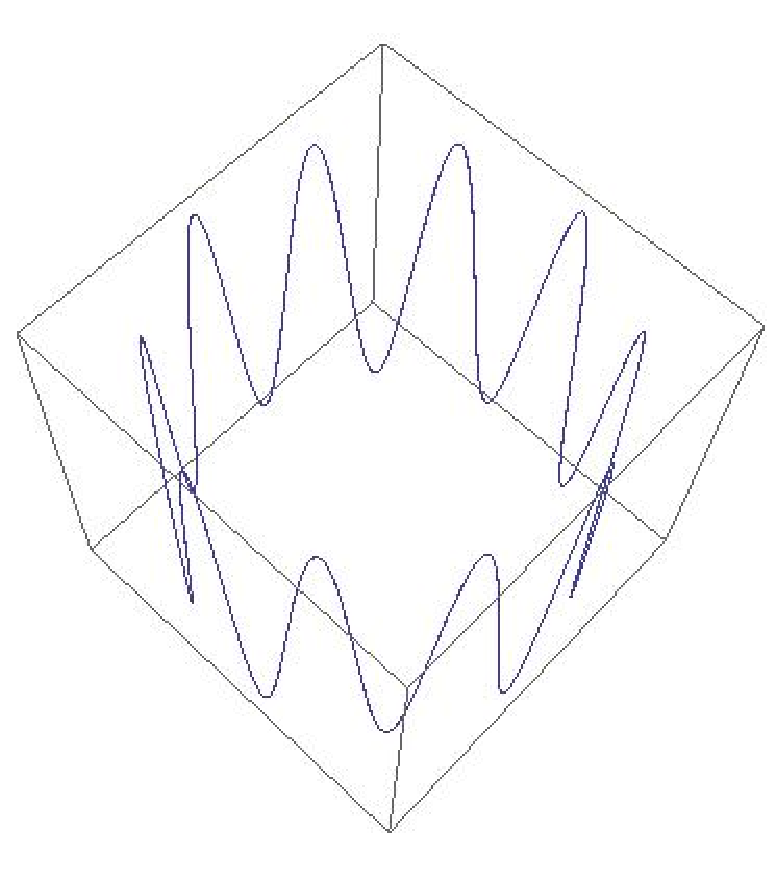
\psfig{file=jpegs/chapter-optical_lattice/fig1.eps,height=3.0in, width=5.0in}
 \caption{Representative diagram of a 'ringed lattice' with period $N=10$.}
 \label{fig:latticering:chapter-oplattice}
 \end{figure}

The interaction matrix elements (see appendix~\ref{appendix-matelements}) go as $\simeq 1/N$, and we set $N$ to 2. In the absence of external drives or interaction, this system reduces to the 2-quantum pendulum $H_{0i}(\kappa)=p_i^2+\kappa \cos{x_i}$, whose eigenstates are the Mathieu functions, and the eigenvalues are the characteristic functions of the Mathieu equation~\cite{abramowitz:stegun}. This is evidenced by looking at the numerically diagonalized eigenvalues in the absence of drives in Fig~\ref{fig:energylevels:chapter-oplattice}. States with $n>0$ are even parity states and states with $n<0$ are odd-parity states, a symmetry that is preserved if we use Eqn~\ref{eq:freeptcl:chapter-oplattice} for diagonalization. Note that $E_n\rightarrow n^2$ as $\kappa \rightarrow 0$, and $E_n\rightarrow n^2$ for large $|n|$ (the 'continuum' limit far above the pendulum separatrix in the classical phase space~\cite{reichl-appendix}).
%Fig 2
\begin{figure} 
\ 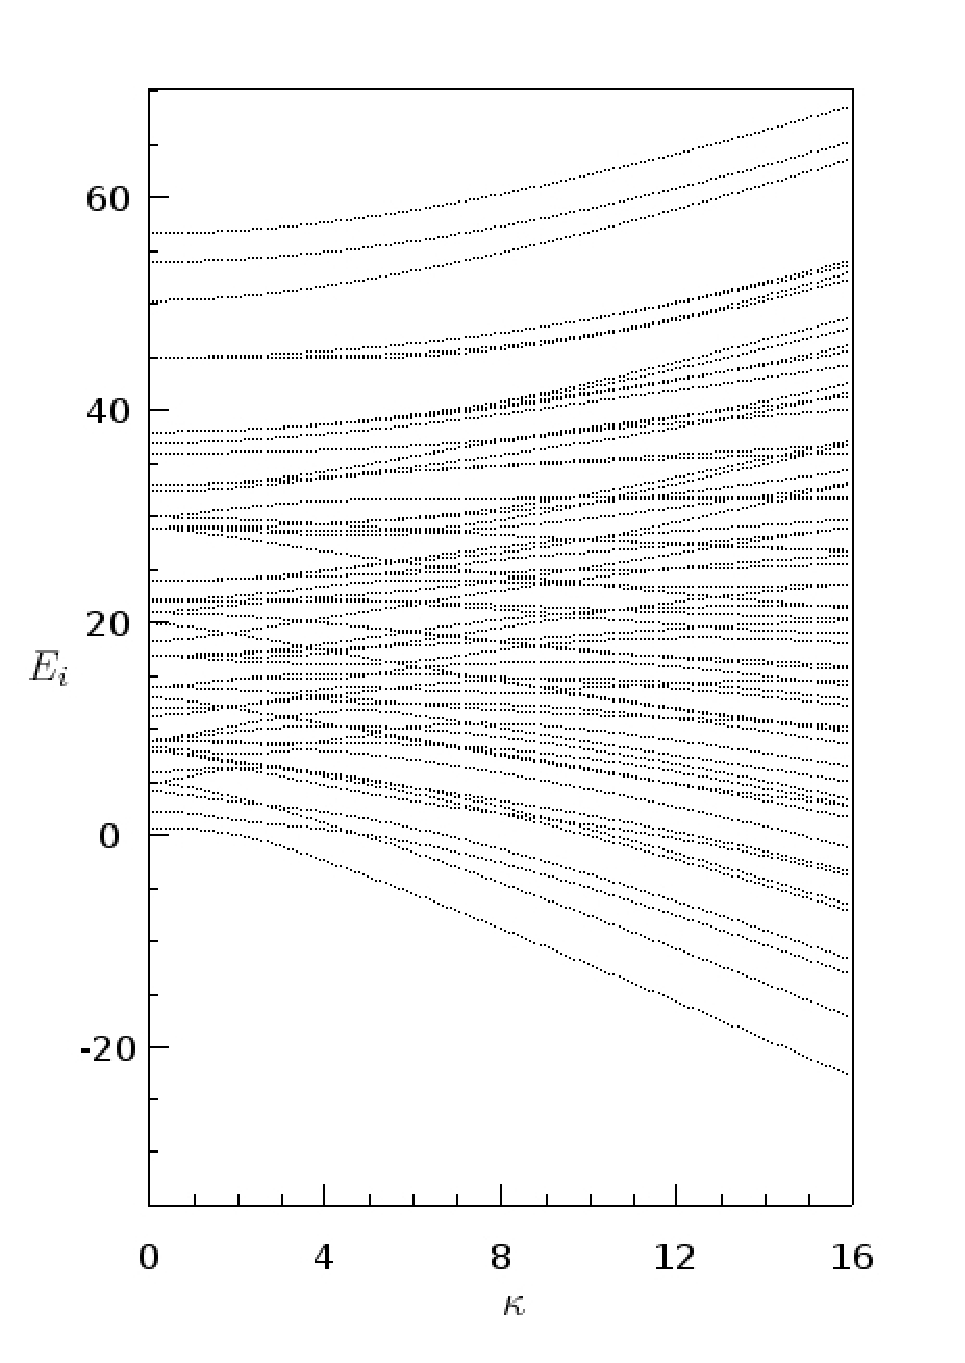
\psfig{file=jpegs/chapter-optical_lattice/fig2.eps,height=5.0in,width=3.0in}
\caption{Energy curves of the first $66$ lowest-energy states of both even and odd parities for the two-boson pendulum for the strongly interacting regime interaction amplitude $u_0=23.0$. Note the similarities with the characteristic functions for the Mathieu equation even for such a strong interaction.}
\label{fig:energylevels:chapter-oplattice}
\end{figure}

\section{\label{sec:3} Quantum Mechanics of the Interacting System}

We numerically diagonalize this Hamiltonian using the same nonadaptive finite element method used in section~\ref{chapter-dblwell:diaghamilt}, where the basis set is given by Eqn~\ref{eq:freeptcl:chapter-oplattice}. The 2-particle boson states of the box system are obtained by symmetrizing the 2-particle states to obtain a complete orthonormal basis of symmetrized 2-boson states:
%
\begin{equation}
{\langle}x_1,x_2\vert n_1,n_2{\rangle} ^{(s)}=\frac{1}{\sqrt{2(1+\delta_{n_1,n_2})}} 
[{\langle}x_1|n_1\rangle{\langle}x_2|n_2\rangle +{\langle}x_1|n_2\rangle{\langle}x_2|n_1\rangle ].
\label{eq:symm:chapter-oplattice}
\end{equation}
These states are then used to create a Hamiltonian matrix from Eqn.~\ref{eq:hamscale:chapter-oplattice}. The eigenvalues $E_i$ and eigenvectors $\vert E_i \rangle$ of the Hamiltonian matrix were determined numerically using the appropriate subroutine for diagonalizing real symmetric matrices in the GNU Scientific Library~\cite{galassi:gsl}. 


\subsection{The Strongly Interacting Regime}
As detailed in appendix~\ref{appendix-tof} for the double well problem, we wish to identify a 'strongly interacting regime' which will consist of a very strongly repulsive system and a moderate well depth. We define the 'strongly interacting factor' for this system, $\gamma$, as 
\begin{equation}
\gamma \equiv \frac{u_0}{E}.
\end{equation}
Here, $E$, the energy of the state, is a measure of the ability of the bosons to tunnel across from one well to another. When $\gamma \rightarrow \infty$, we reach the 'strongly interacting' regime where the system behaves line a Tonks gas, and the interaction completely dominates the system~\cite{tonks:gas}. The order parameter used to determine this is $p_i/{\delta l}$, where
\begin{equation}
p_i \equiv \delta l \int dx| \langle x,x | E_1 \rangle |^2.
\end{equation}
The order parameter $p_i$ is the total probability that the two particles lie arbitrarily close to each other within $\delta l$, and $i$ divides the $\gamma$-space into different regions of interest. Figure~\ref{fig:oplattice_tonksplot:chapter-oplattice} shows the plot of this  one dimensional probability density as a function of the strongly interacting factor. As expected, it vanishes for arbitrarily large values of $\gamma$, since the strong repulsions prevent two particles from being together. The transition to this regime is marked by a discontinuous change in the exponential decay of $p_i$ at $\gamma \sim 1.25$. The data points have been fitted to exponential decays,$\left( p_i/{\delta l} \right)=\left( p^0_i/{\delta l} \right) e^{-(\gamma/\gamma^0_i)}$ ,  by the use of numerical nonlinear least-squares algorithms. Here, $i$ denotes the region where the decay rate $\gamma^0$ appears to be fixed. We choose a value of $u_0=23.0$ for this particular value of $\kappa=4.9376435$ such that $\gamma=2.77465$, placing the system well in the region marked by $p_2$, and at a value of $p << p^0_1/e$.

%Fig 4
\begin{figure} 
\hspace*{-0.2in}
\ 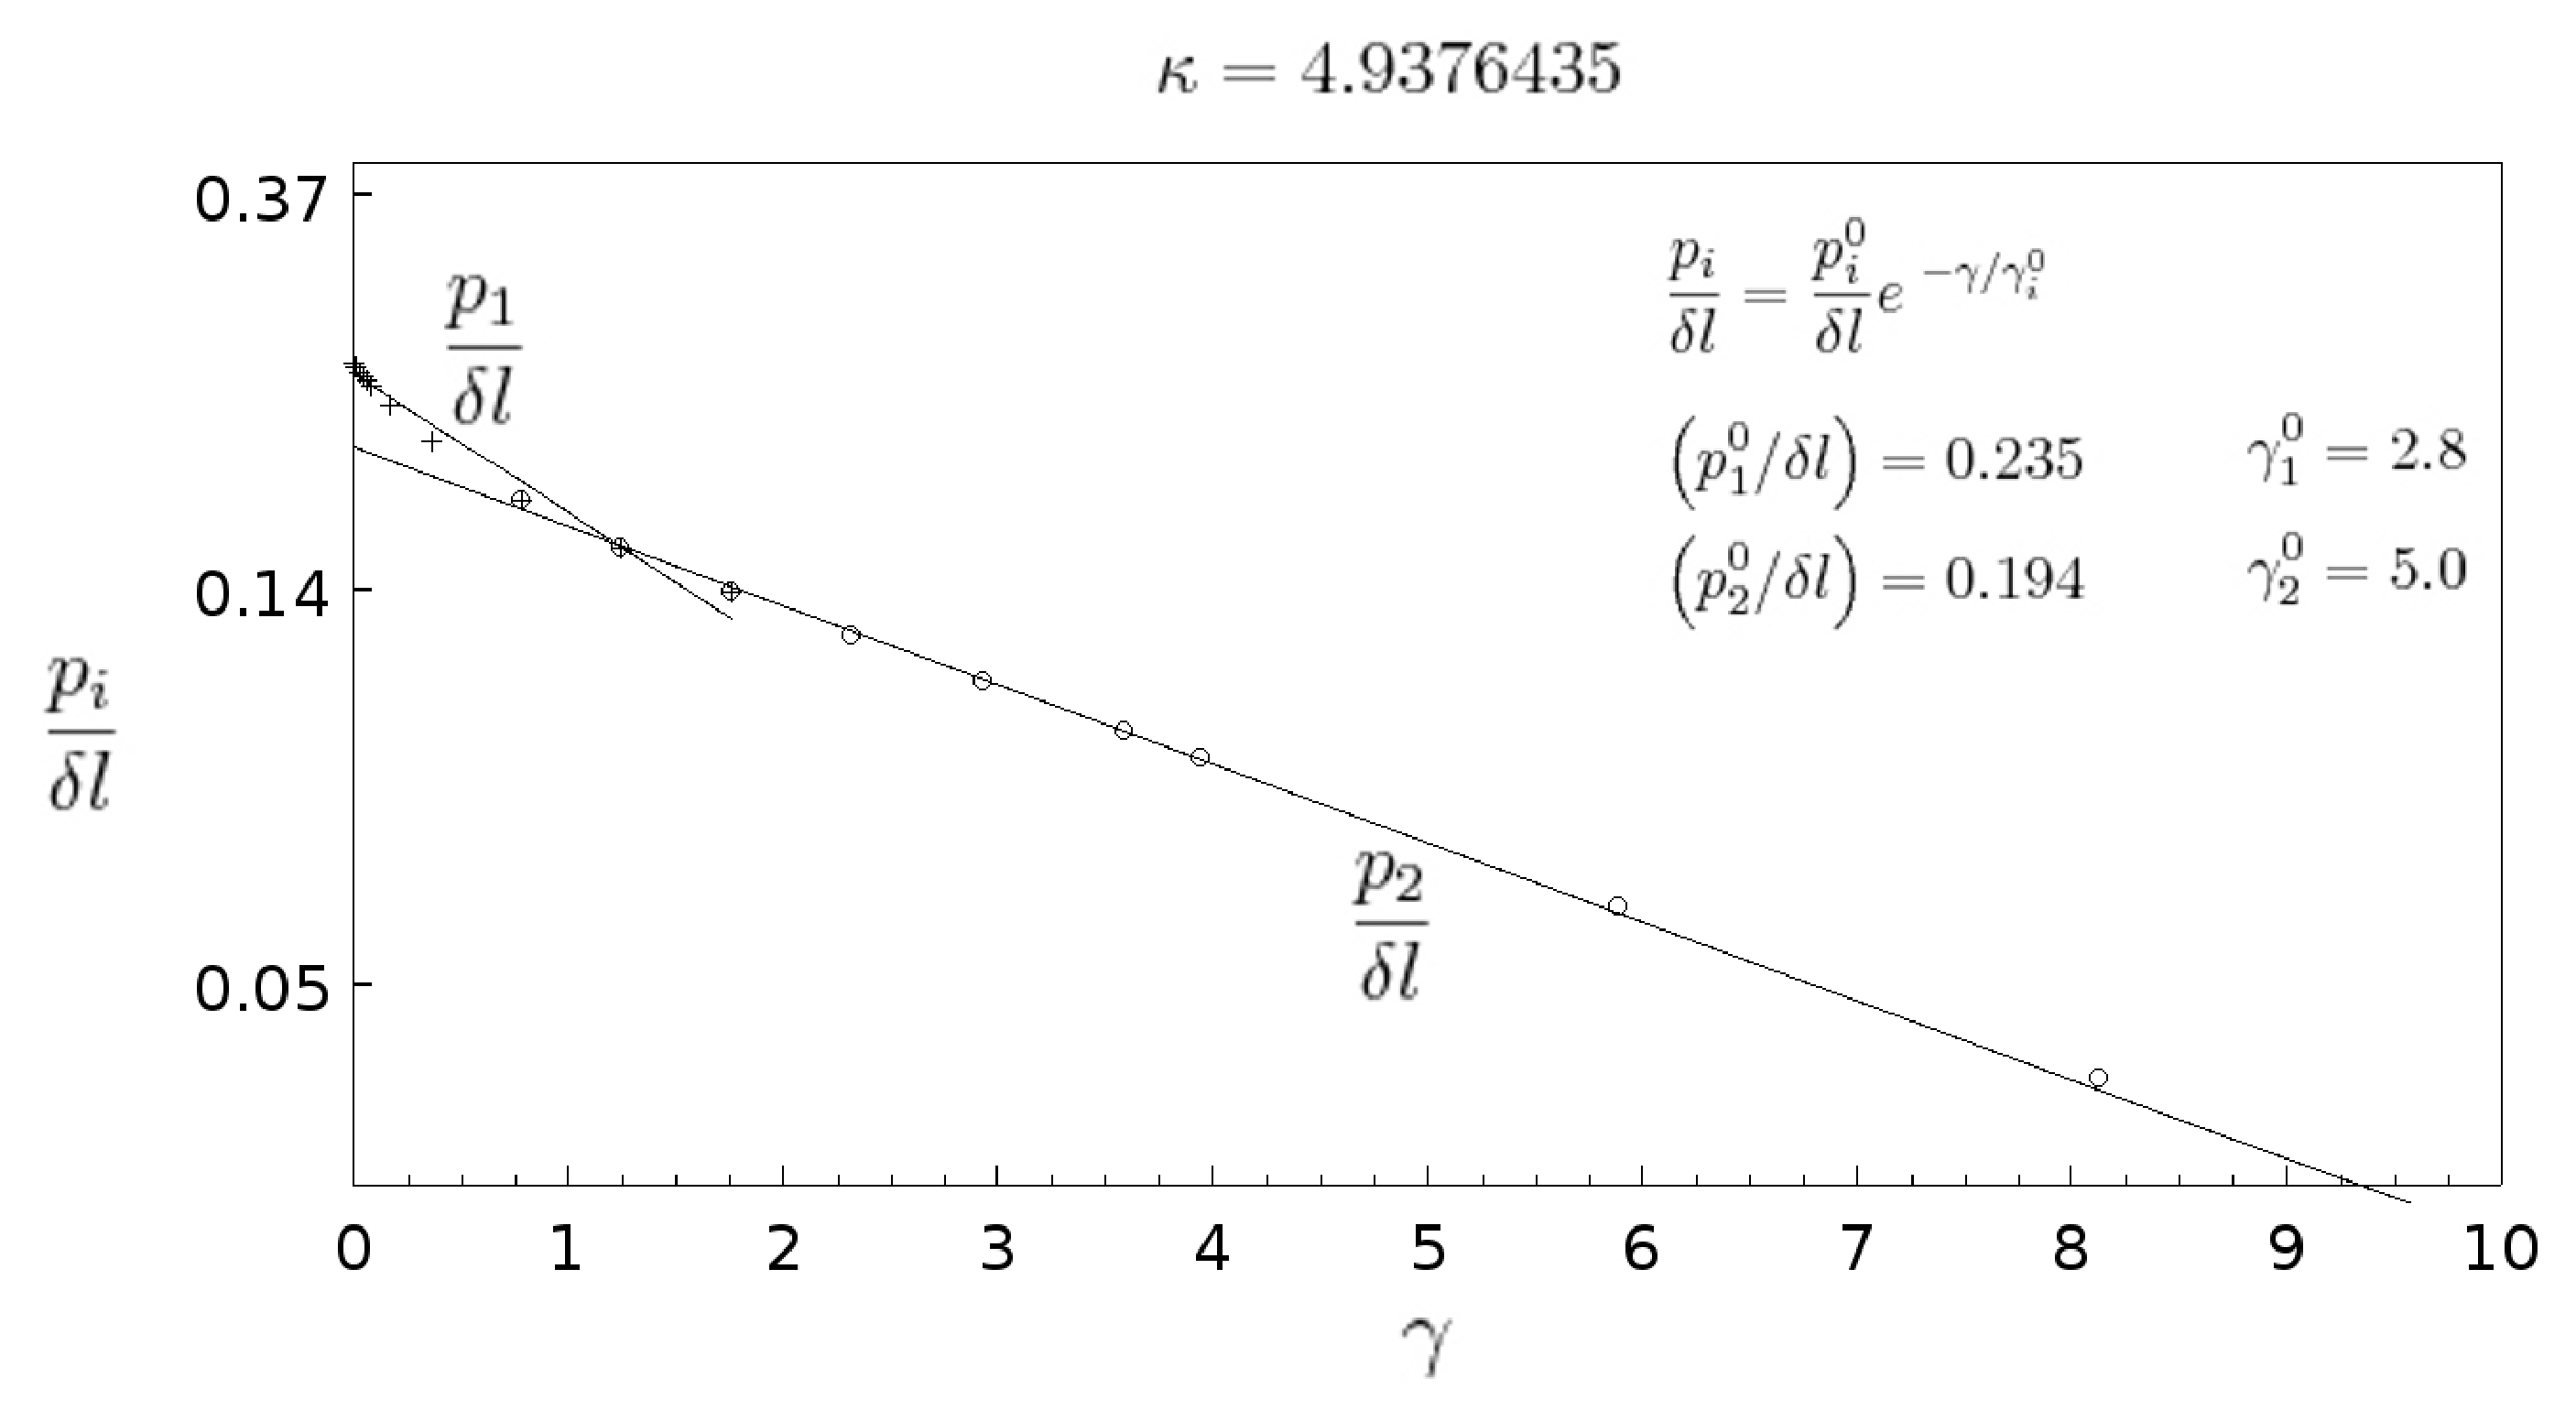
\psfig{file=jpegs/chapter-optical_lattice/fig4.eps,height=3.8in,width=5.7in}
\caption{Semi-logarithmic plot of the probability $\psi_i$ of two particles having the same position, as a function of the strongly interacting parameter $\gamma$ for a constant $\kappa=4.9376435$. The decay rate of $\psi$ changes sharply across $2$  regions, labeled by the index $i$. The data points (indicated by crosses and circles) have been fitted to exponential decay rates at each region (indicated by lines).The legend provides the numerically fitted values of the decay rates $\gamma^0_i$.}
\label{fig:oplattice_tonksplot:chapter-oplattice}
\end{figure}

\subsection{Energy Eigenstates}
Figures~\ref{fig:wavefunctions:chapter-oplattice}.a through~\ref{fig:wavefunctions:chapter-oplattice}.e are the probability distribution plots for the states $\langle x_1, x_2 | E_1 \rangle$, $\langle x_1, x_2 | E_3 \rangle$, $\langle x_1, x_2 | E_4 \rangle$,$\langle x_1, x_2 | E_5 \rangle$, and $\langle x_1, x_2 | E_{15} \rangle$ respectively at the value of $\kappa$ obtained in the section above. We chose these states because these transitions have the largest  amplitudes of $\cos{x}$, thus exhibiting significant Rabi oscillations. Note the presence of scarring in the wavefunctions of $|E_{14}\rangle$  and $|E_{18}\rangle$, where centroids seem to follow the classical trajectories for two bosons at that energy.

%Fig 5
\begin{figure} 
\ 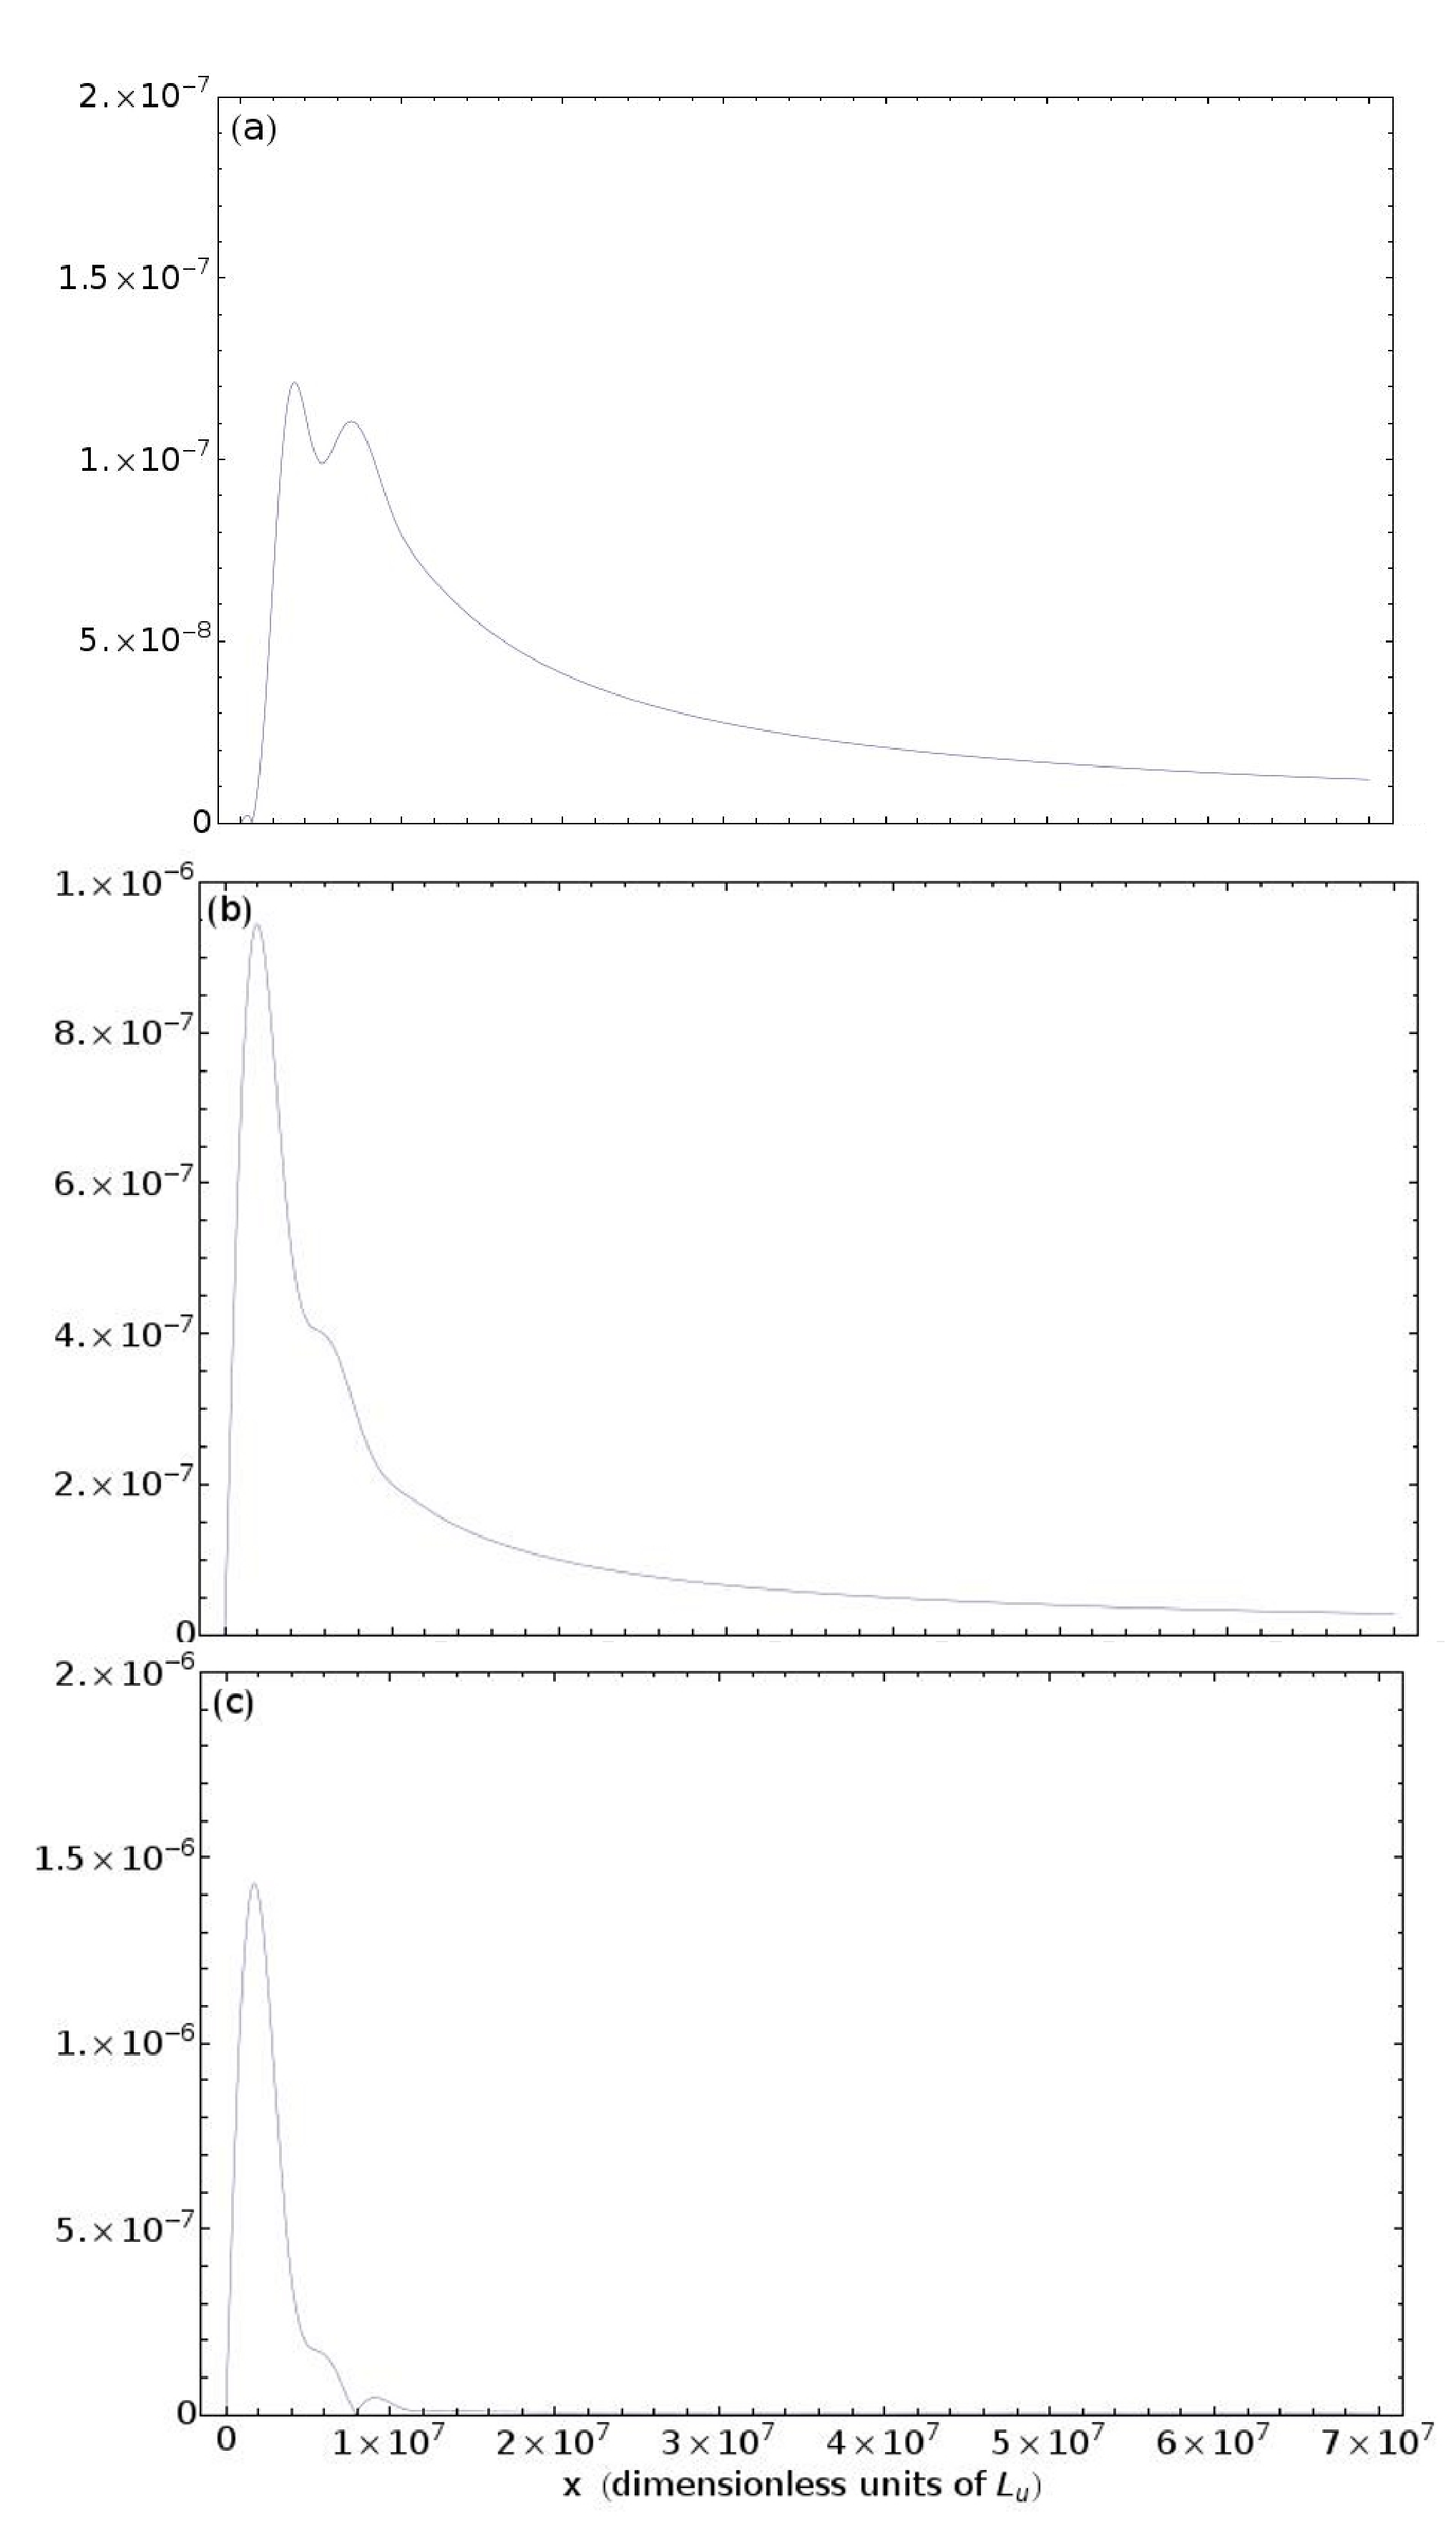
\psfig{file=jpegs/chapter-optical_lattice/fig5.eps,height=7.0in,width=2.0in}
\caption{Wavefunction plots for states 1, 3, 4, 5 , and 15}
\label{fig:wavefunctions:chapter-oplattice}
\end{figure}

\section{\label{sec:4} STIRAP Ladder, First Pulse $4 \leftrightarrow 15$, Second Pulse $1 \leftrightarrow 4$}
We now subject the system to a five resonance drive similar to the three-resonance drive done by Luter and Reichl~\cite{luter:reichl:3res} and Holder and Reichl~\cite{holder-reichl:avoidedcross} via STIRAP, using the five-resonance Hamiltonian defined by Eqn~\ref{eq:fiveres:chapter-oplattice}. In dimensionless form, this is 
\begin{eqnarray}
H=H_1(x_1,t)+H_2(x_2,t)+u_0 \delta(x_1-x_2) \\
H_i(x_i,t)=p_i^2 +\kappa \cos{x_i}+ \lambda_f \cos{x_i } \cos{ \omega_f t}+\lambda_s \cos{x_i} \cos{ \omega_s t}.
\end{eqnarray}
The drive for the five resonance Hamiltonian consists of two extra pairs of frequency-offset lasers, but drifting in opposite directions with speed $\omega_{f,s}$. The amplitudes of the lattices, $\lambda_{f,s}$, are slowly varying in time. Thus, 

\begin{equation}
H_i(t:t_{fix}) = \lambda^0  \cos{x_i} \left[ \lambda_f(t_{fix})\cos{\omega_f t} + \lambda_s(t_{fix}) \cos{\omega_s t}\right]
\end{equation}
for each particle. Here, 
\begin{equation}
 \lambda_{f,s}(t_{fix}) = e^{-(t_{fix}-t_{f,s})^2/4t^2_d},
 \label{eq:stirap:amp:chapter-oplattice}
\end{equation}
thus reproducing the time modulated radiation pulses characteristic of STIRAP as seen in sections~\ref{chapter-intro:section:stirap} and ~\ref{chapter-dblwell:section:stirap}. The driving frequencies $\omega_f=(E_{15}-E_4)$ and $\omega_s=(E_4-E_1)$. Thus, we are doing a ladder transition of the type $1\rightarrow 4 \rightarrow 15$ for a chosen value of $\kappa$ (see Fig~\ref{fig:stirap:chapter-oplattice}). 

If the two driving frequencies are rational factors ie $\omega_f/\omega_s = n_f/n_s$ for least common factor integers $n_{f,s}$, and the adiabatic time $t_{fix}$ varies slowly compared to the time period $T$ where
\begin{equation}
T=\pi \left(\frac{n_f}{\omega_f}+\frac{n_s}{\omega_s}\right),
\end{equation}
then the drive is time periodic and Floquet's theorem guarantees solutions of the type 
\begin{equation}
 |\psi_\alpha(t)\rangle=e^{-i\Omega_\alpha t}|\phi_\alpha(t)\rangle.
\end{equation}
Here, $|\phi_\alpha(t)\rangle$, the Floquet eigenstate(s) are $T$-periodic and $\Omega_\alpha$s are the Floquet eigenvalue(s), exactly as seen in  subsection~\ref{chapter-dblwell:section:qdynamics:subsec:floquet}. The value of $\kappa$ has been adjusted (see Fig~\ref{fig:stirap:chapter-oplattice}) to achieve commensurability of frequencies without requiring any detuning.

The matrix elements of Floquet evolution operator, $U_F(T)$, is given by
\begin{equation}
U_F(T) = \sum_{\alpha} e^{-i\Omega_{\alpha}T}|\phi_{\alpha}(0)\rangle\langle \phi_{\alpha}(0)|,
\end{equation}
%
and can be calculated numerically by integrating each column of the unit operator as the initial conditions by time $T$. This is done using an $8^{th}$ order Runge-Kutta Prince Dormand algorithm~\cite{rkutta:pd} from the GNU Scientific Library~\cite{galassi:gsl}, and the matrix diagonalized using a parallelized LAPACK library through the Scalable Library for Eigenvalue Problem Computations (Slepc)~\cite{slepc}. The eigenvalues, $e^{-i\Omega_{\alpha}T}$ can be used to obtain $\Omega_{\alpha}$ modulo one Floquet photon in the Brillouin zone as shown in subsection~\ref{chapter-dblwell:section:qdynamics:subsec:floquet}. A profile of the Floquet eigenvalues as a function of $t_{fix}$ provides a complete picture for the dynamics of the STIRAP process. As we have shown for the double well case in section~\ref{chapter-dblwell:section:stirap}, the Floquet eigencurves can be labeled by their dominant eigenstate or 'support state' (the energy eigenstates with which they are isomorphic at $t_{fix}=0$).
%Fig 3
\begin{figure} 
\ 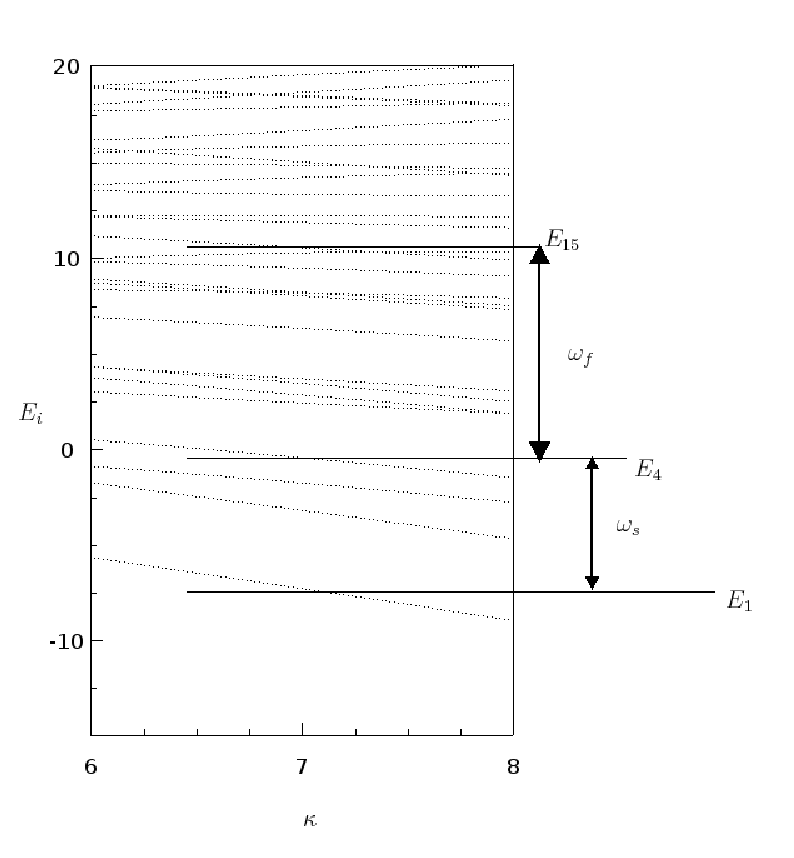
\psfig{file=jpegs/chapter-optical_lattice/fig3.eps,height=5.0in,width=5.0in}
\caption{Magnified view of energy curves shown in Fig~\ref{fig:energylevels:chapter-oplattice} with the value of $\kappa=7.287781$ chosen for the strongly interacting regime included. The levels being connected by STIRAP for this particular value of $\kappa$ are indicated. The value of $\kappa$ has been adjusted so that $\frac{\omega_f}{\omega_s}=\frac{3}{2}$}
\label{fig:stirap:chapter-oplattice}
\end{figure}

We chose to vary the STIRAP amplitudes as shown in Fig~\ref{fig:stirap_amps:chapter-oplattice}, with $\lambda_0=0.2$, $t_f=(1/3) t_{tot}$, $t_s=(2/3)t_{tot}$, and the pulse widths $t_d=(1/14)t_{tot}$. Here $t_{tot}$ defines the total time scale for both pulses, and $t_{fix}$ is expressed in units of $t_{tot}$ unless otherwise stated, the $t_{tot}$ dependence on $\Omega_\alpha$ being negligible~\cite{na-reichl:pbox}~\cite{na-reichl:mol-rot}~\cite{na-reichl:isomer}. Figure~\ref{fig:floquet_quasi_0.2:chapter-oplattice} shows the Floquet eigenvalues of the relevant Floquet eigenstates as the system evolves in adiabatic time. The relevant eigenstates are the ones isomorphic to the states connected by the STIRAP pulses viz. $|E_1\rangle$, $|E_4\rangle$, and $|E_{15}\rangle$. We notice that the eigenvalues are degenerate at $t_{fix}=0$ and $t_{fix}=t_{tot}$ as expected. We also note a higher order resonance that brings $|E_{18}\rangle$ into the degenerate subspace. The Floquet states and corresponding quasienergies are labeled alphabetically as follows:
\begin{enumerate}
 \item
The eigenphase whose corresponding Floquet eigenstate is supported by the undriven  state $|E_{18}{\rangle}$  at $t_{fix}=0$ is labeled as $\Omega_A$ and the Floquet eigenstate as $|\phi_A\rangle$.
\item
The eigenphase whose corresponding Floquet eigenstate is supported by the undriven state $\frac{1}{\sqrt{2}}\left[|E_4\rangle - |E_{15}\rangle \right]$ at $t_{fix}=0$ is labeled as $\Omega_B$ and the Floquet eigenstate as $|\phi_B\rangle$.
\item
The eigenphase whose corresponding Floquet eigenstate is supported by the undriven state $\frac{1}{\sqrt{2}}\left[|E_4\rangle + |E_{15}\rangle \right]$ at $t_{fix}=0$  is labeled as $\Omega_C$ and the Floquet eigenstate as $|\phi_C\rangle$.
\item 
The eigenphase whose corresponding Floquet eigenstate is supported by the undriven ground state $|E_1{\rangle}$  at $t_{fix}=0$ is labeled as $\Omega_D$ and the Floquet eigenstate as $|\phi_D\rangle$.
\end{enumerate}
%Fig 6
\begin{figure} 
\ 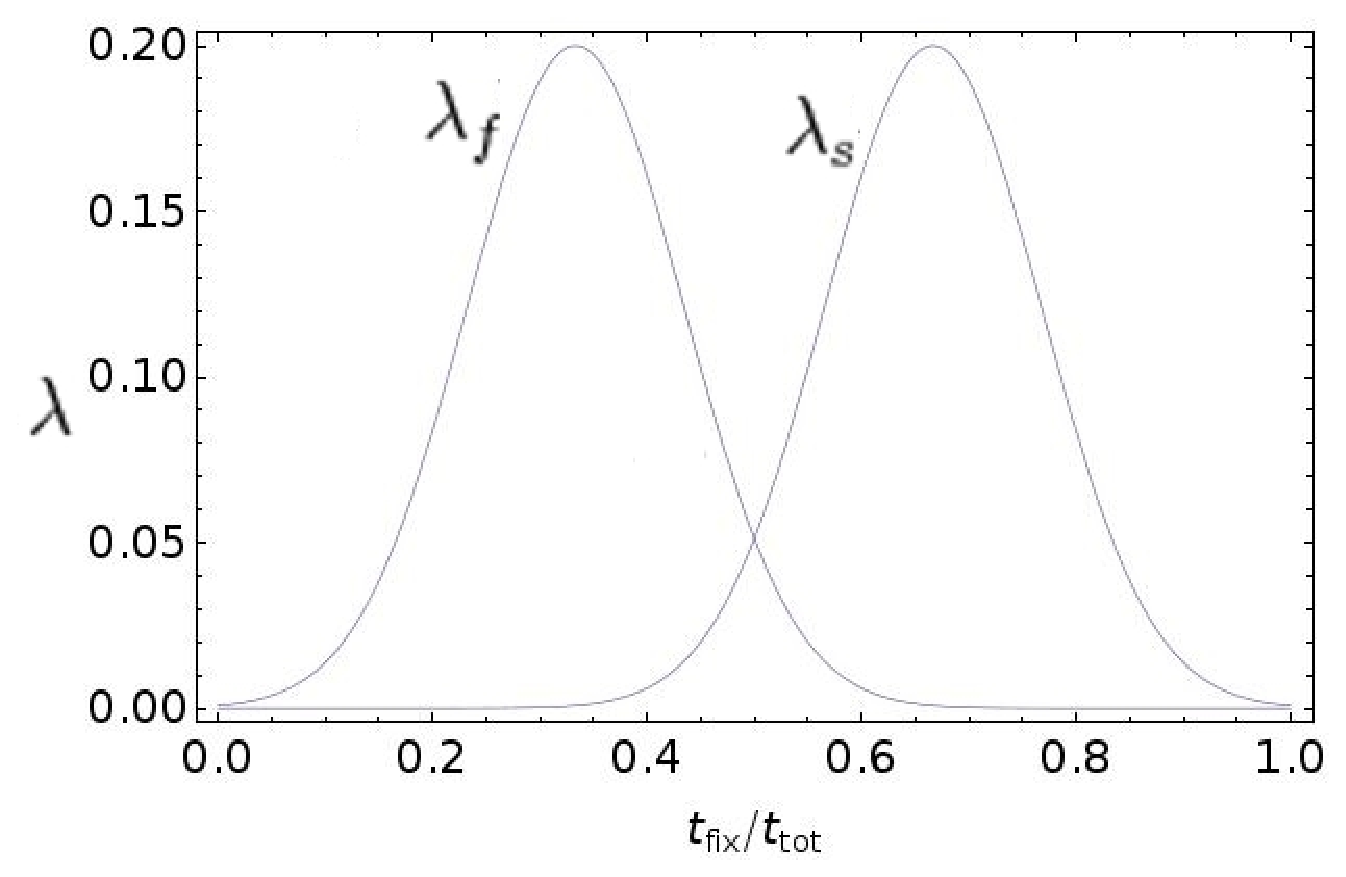
\psfig{file=jpegs/chapter-optical_lattice/fig6.eps,height=3.0in,width=5.0in}
\caption{The amplitudes $\lambda_{f,s}$ of the STIRAP pulses as a function of time with $\lambda_0=0.2$ (see Eqn~\ref{eq:stirap:amp:chapter-oplattice}). The first pulse (in time)  connects the intermediate state to the final state of the STIRAP process. All units are dimensionless. The second pulse (in time)  connects the initial state and the intermediate state. The total time $t_{tot}$ is chosen arbitrarily, but the centroids of the pulses are kept at $\frac{t_f}{t_{tot}}=\frac{1}{3}$,$\frac{t_s}{t_{tot}}=\frac{2}{3}$,$\frac{t_d}{t_{tot}}=\frac{1}{14}$,where $t_{f,s}$ are the centroids of the first and second pulses respectively, and $t_d$ is the width of the pulses.}
\label{fig:stirap_amps:chapter-oplattice}
\end{figure}

Thus, the system, if evolving adiabatically, stays in $\Omega_D$ at all times, and avoids all avoided crossings that it encounters during STIRAP. We notice signs of traditional $3$-level avoided crossing for the system at $t_{fix}\simeq 0.5$ $t_{tot}$ in Fig~\ref{fig:floquet_quasi_0.2:chapter-oplattice}. However, we notice additional avoided crossings in $\Omega_D$ that will affect the transitions in the system. First, $\Omega_D$ appears to undergo an avoided crossing with $\Omega_A$ at $t_{fix}\simeq 0.45$ $t_{tot}$, exchanging characteristics of $|\phi_D\rangle$ in the process. The traditional 3-level STIRAP transition occurs after this event. Before the dynamics is complete, however, another avoided crossing occurs between $\Omega_D$ and $\Omega_A$, also causing the character of $|\phi_D\rangle$ in the process. Thus, the final outcome of a stimulated Raman adiabatic passage will be very different from traditional STIRAP if the crossings are navigated by adiabatic passage. The dependence of $|\phi_A\rangle$ through $|\phi_D\rangle$ on the unperturbed energy eigenstates is shown in Fig~\ref{fig:floquet_states_0.2:chapter-oplattice}. The influence of the avoided crossings is clearly seen. The final outcome is a linear superposition of the type $\frac{1}{\sqrt{2}}(|E_1\rangle \pm |E_4\rangle)$. These avoided crossings are manifestations of classical chaos in the quantum dynamics similar to the ones seen for the double well system in chapter~\ref{chapter-dblwell}.
  
The dynamics can be analyzed in more detail by using the Landau-Zener formula to calculate the probability of a transition at an avoided crossing. The probability $P_{\alpha\beta}$ for an avoided crossing between two Floquet eigenphases $\Omega_{\alpha}$ and $\Omega_{\beta}$ to be crossed  is given by (see Eqn~\ref{eq:lzformula:chapter-intro})
\begin{equation}
P_{\alpha \beta}=\exp\left[-\frac{\pi ({\delta \Omega_{\alpha \beta}})^2}{2\Gamma_{\alpha \beta}}\right],
\label{eq:landauzener:chapter-oplattice}
\end{equation}
%
%
where $\delta\Omega_{\alpha\beta}$ is the (minimum) spacing  between $\Omega_\alpha$ and $\Omega_\beta$ at the avoided crossing and $\Gamma_{\alpha\beta}$   is the magnitude of the  rate of change (slope) of the Floquet eigenphases in the immediate neighborhood of the avoided crossing. Thus,
%
\begin{equation}
\Gamma_{\alpha\beta} = {\biggl|} \frac{d\Omega_\alpha}{dt} - \frac{d\Omega_\beta}{dt}{\biggr|},
\label{eq:gamma:chapter-oplattice}
\end{equation}
%
where  $\frac{d\Omega_\alpha}{dt}$ is the slope of the  eigenphase curve $\Omega_\alpha$ in the neighborhood of the avoided crossing. We follow the derivation of the Landau-Zener formula for the double well system in previous chapters to get 
\begin{equation}
P_{\alpha \beta}=\exp\left[-t_{tot}{\gamma}_{\alpha,\beta} \right].
\label{eq:lanzen:chapter-oplattice}
\end{equation}
%
where ${\gamma}_{\alpha,\beta}=\frac{\pi ({\delta \Omega_{\alpha \beta}})^2}{2{\bar \Gamma}_{\alpha \beta}}$. 

In order for a crossing to be avoided instead of crossed, $P_{\alpha\beta}\approx 0$, and the actual time scale of the STIRAP must be adjusted accordingly. Thus, the transfer probability $P_{\alpha \beta}$ will be very small if $t_{tot}>1/{\gamma}_{\alpha,\beta}$. 
Figures~\ref{fig:floquet_states_0.2:mag:chapter-oplattice}.a and~\ref{fig:floquet_states_0.2:mag:chapter-oplattice}.b show magnified plots of the eigenphases at the two avoided crossings described above. For the first $AD$ avoided crossing shown in Fig~\ref{fig:floquet_states_0.2:mag:chapter-oplattice}.a, we estimate the gap $\delta \Omega_{AD}$ to be $3.67 \times 10^{-4}$, and $\Gamma_{AD}$ to be $0.0155$, rendering $\frac{2\gamma_{AD}}{\pi}$ to be $8.6803 \times 10^{-7}$. Thus $t_{tot}>7.334 \times 10^{4}$. Similarly, for the second $BD$ avoided crossing (Fig~\ref{fig:floquet_states_0.2:mag:chapter-oplattice}.b), $\delta \Omega_{BD}\simeq 1.984 \times 10^{-3}$, and  $\Gamma_{BD}\simeq 0.135$, concluding that $t_{tot}>2.184 \times 10^4$. For $^{85}Rb$, we noted in section~\ref{chapter-intro:section:lightatom:subsec:2lvl} that the $D_2$ transition line is is about $780$ $nm$ (see Fig~\ref{fig:rblevels}). The recoil frequency, $ \omega_r$ is thus about $24$ $KHz$. The characteristic time scale here is $1/(4\omega_r)$, or $1.03 \times 10^{-5}$ seconds. We can plug this value to the minimum value(s) of $t_{tot}$ to get the actual time. Thus, for the $^{85}Rb$ atom, we get $t_{tot}>0.756$ $sec$ for the $AD$ crossing and $t_{tot}>0.225$ $sec$ for the $BD$ crossing. Thus, the $BD$ crossing is automatically avoided if the $AD$ crossing is avoided, making the most rapid required time scale for both chaos assisted adiabatic passages to be $0.756$ seconds. If the time scale for the stirap is faster than $0.225$ seconds, then neither crossing is avoided and traditional 3-level STIRAP will be seen.
%fig 7
\begin{figure} 
\vspace*{-0.1in}
\ 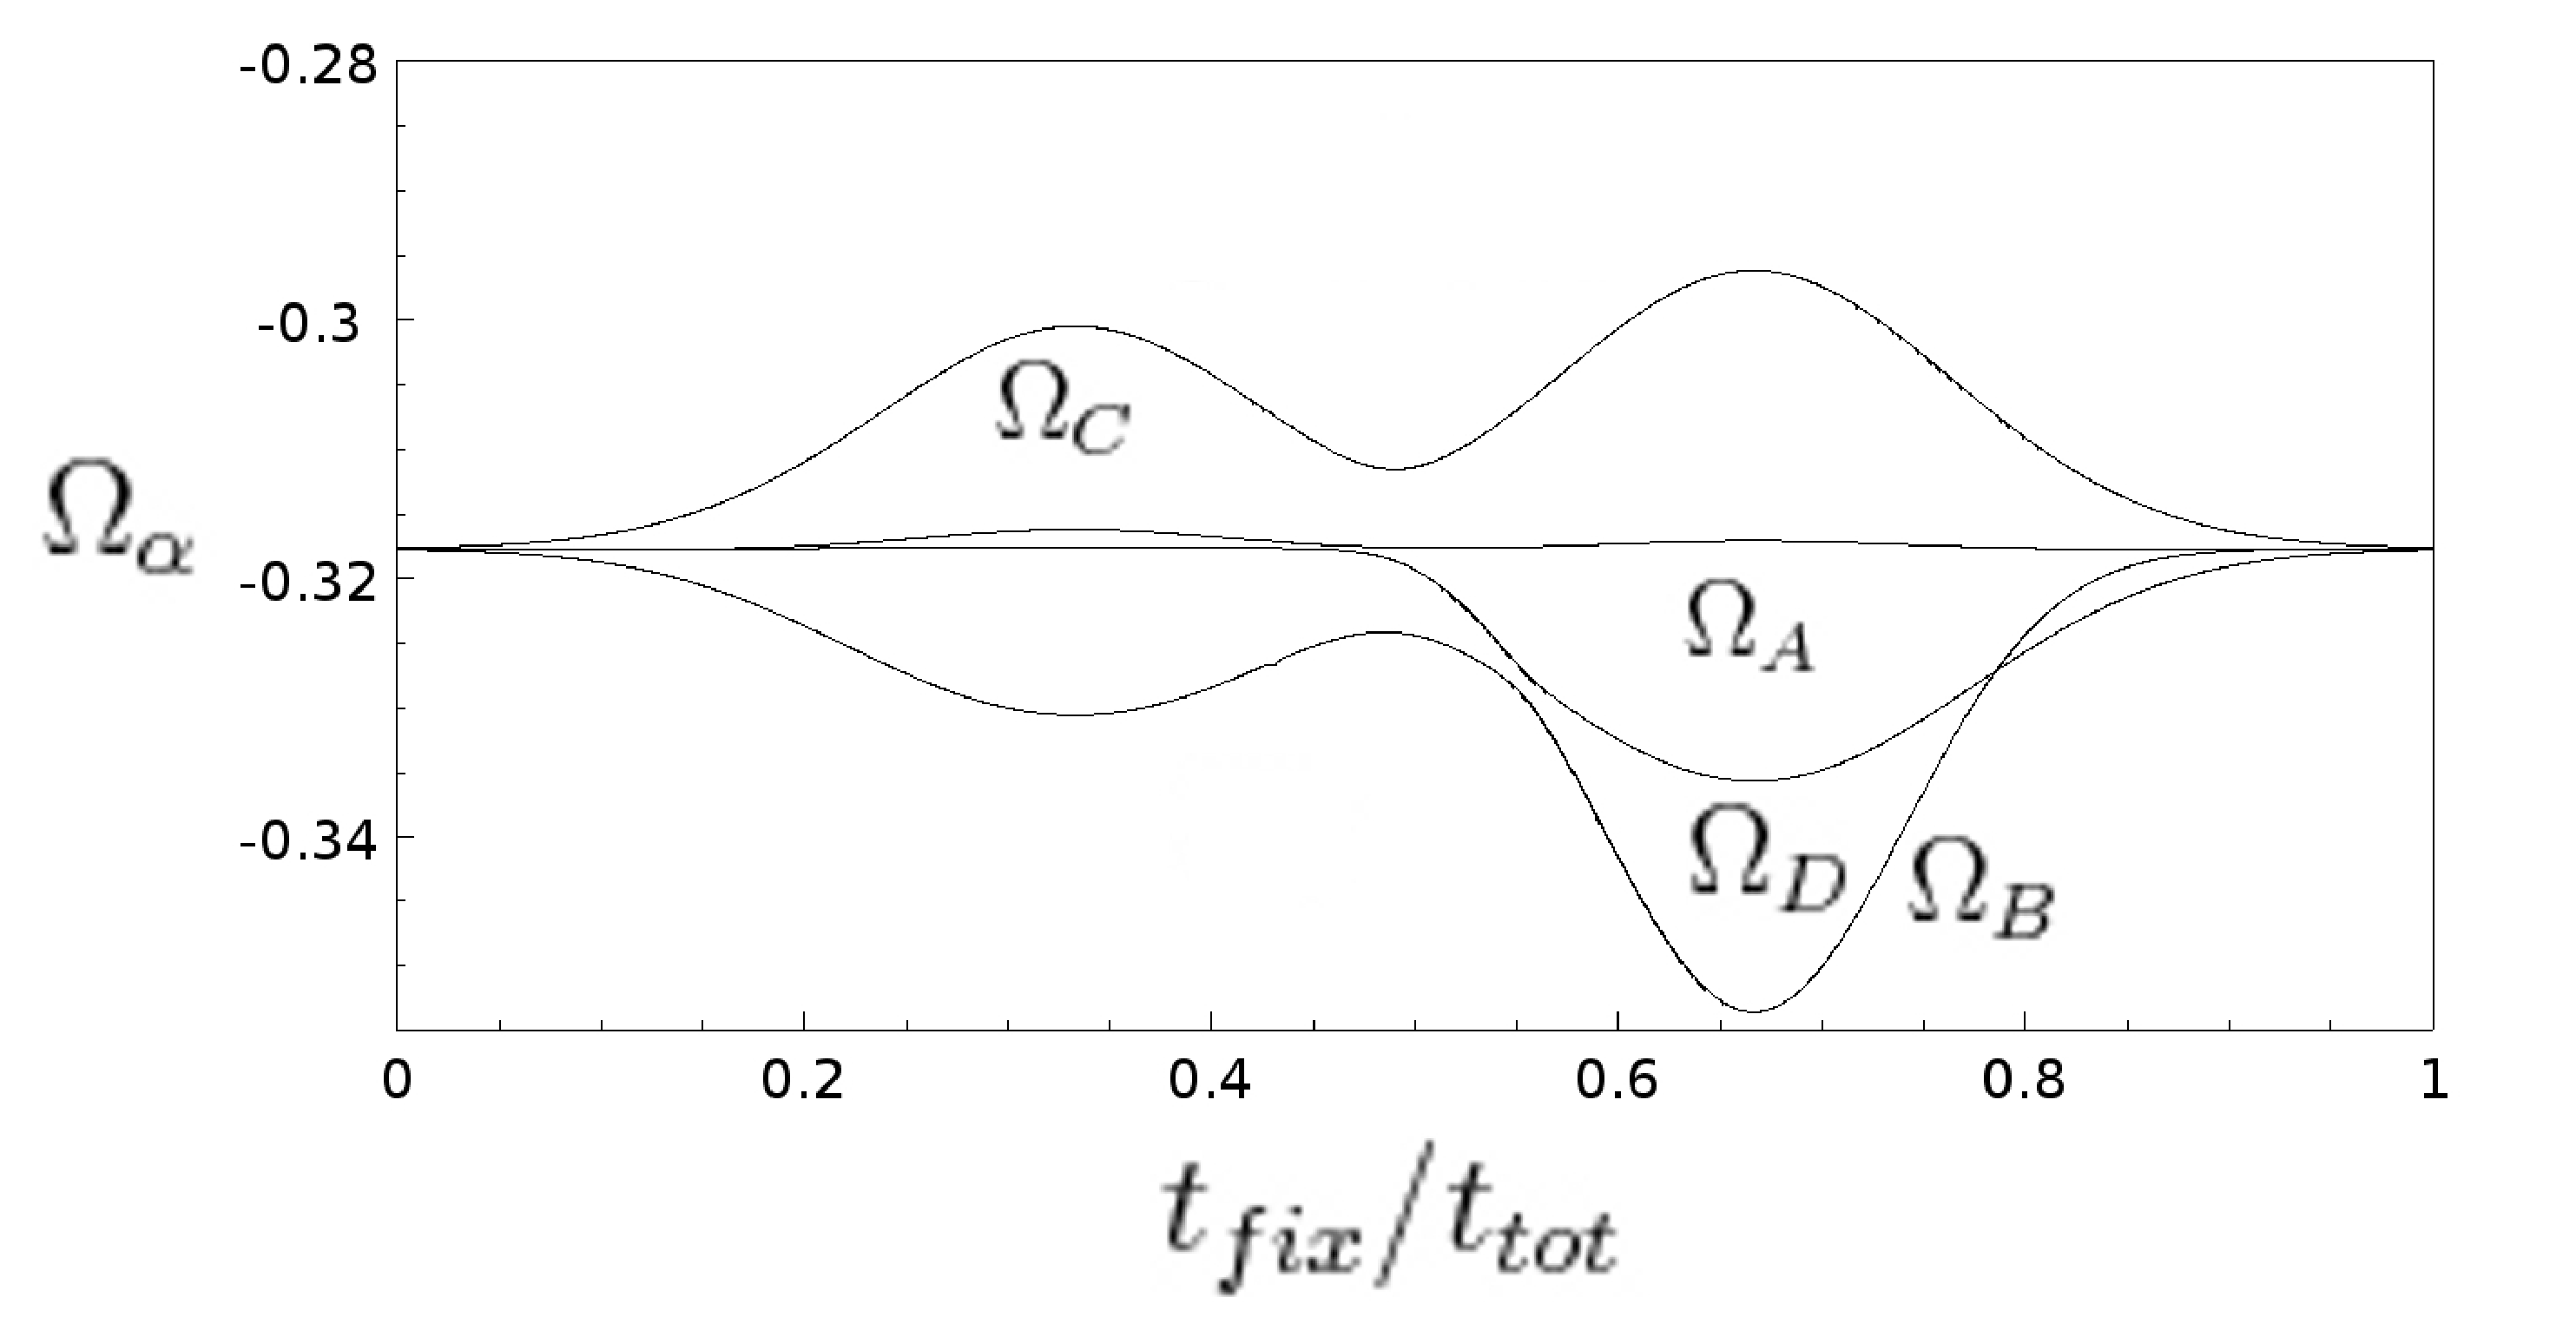
\psfig{file=jpegs/chapter-optical_lattice/fig7.eps,height=3.5in,width=4.6in}
\caption{Floquet quasienergies $\Omega_{\alpha}$ as a function of adiabatic time $t_{fix}/t_{tot}$ for $\lambda^0=0.2$. the labels $\Omega_{A-D}$ denote the floquet quasienergy curves corresponding to the Floquet eigenstates $|\phi_{A-D}\rangle$ respectively. The Brillouin zone is $\left[-\frac{\omega}{2}, \frac{\omega}{2}\right]$}
\label{fig:floquet_quasi_0.2:chapter-oplattice}
\end{figure}
%Fig 8
\begin{figure} 
\ 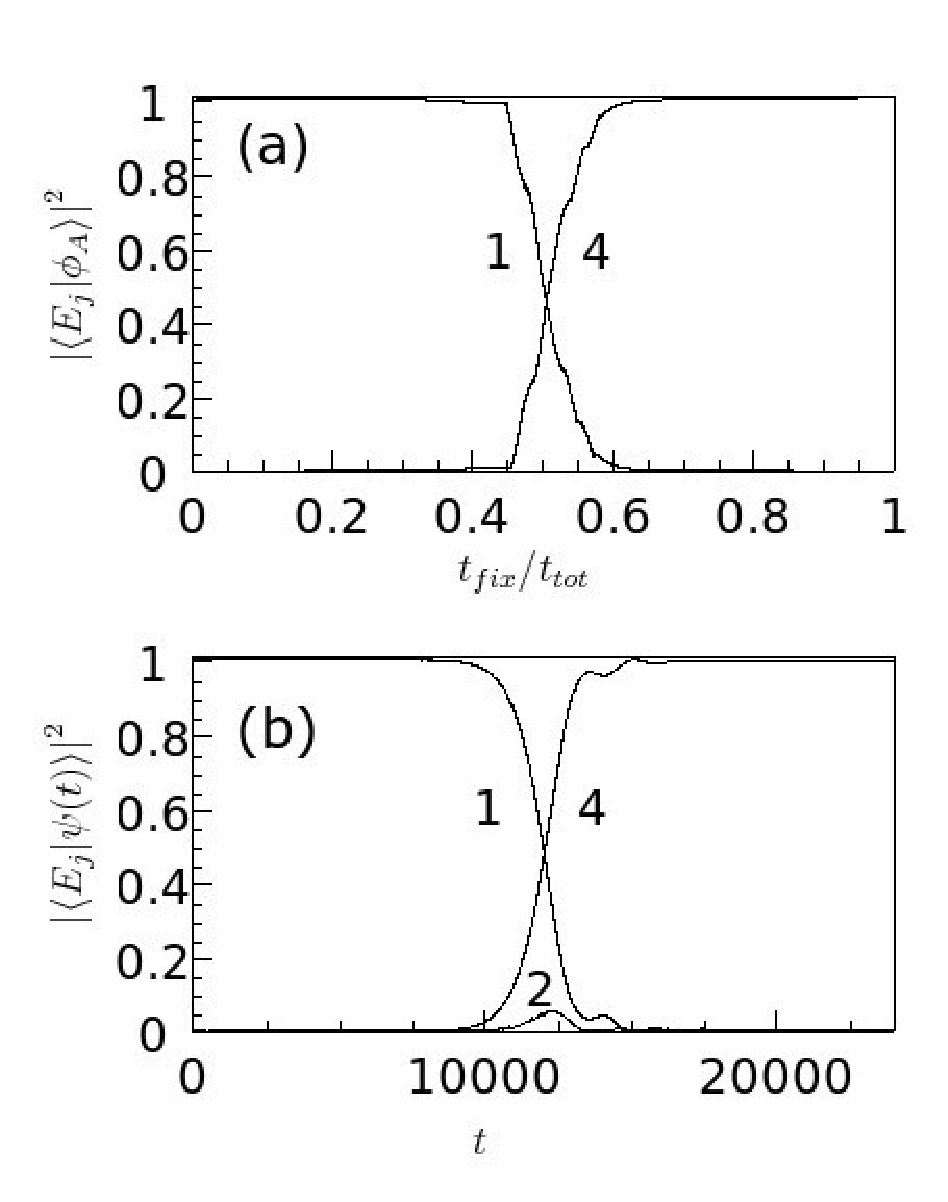
\psfig{file=jpegs/chapter-optical_lattice/fig8.eps,height=6.0in,width=3.0in}
\caption{Plot of the Floquet eigenfunctions $\langle E_i|\phi_{A-D}\rangle$ in the undriven Hamiltonian representation. The components of the Floquet states in each energy level are numbered. Note the influence of the avoided crossings in $|\phi_D\rangle$.}
\label{fig:floquet_states_0.2:chapter-oplattice}
\end{figure}
%Fig 9
\begin{figure} 
\ 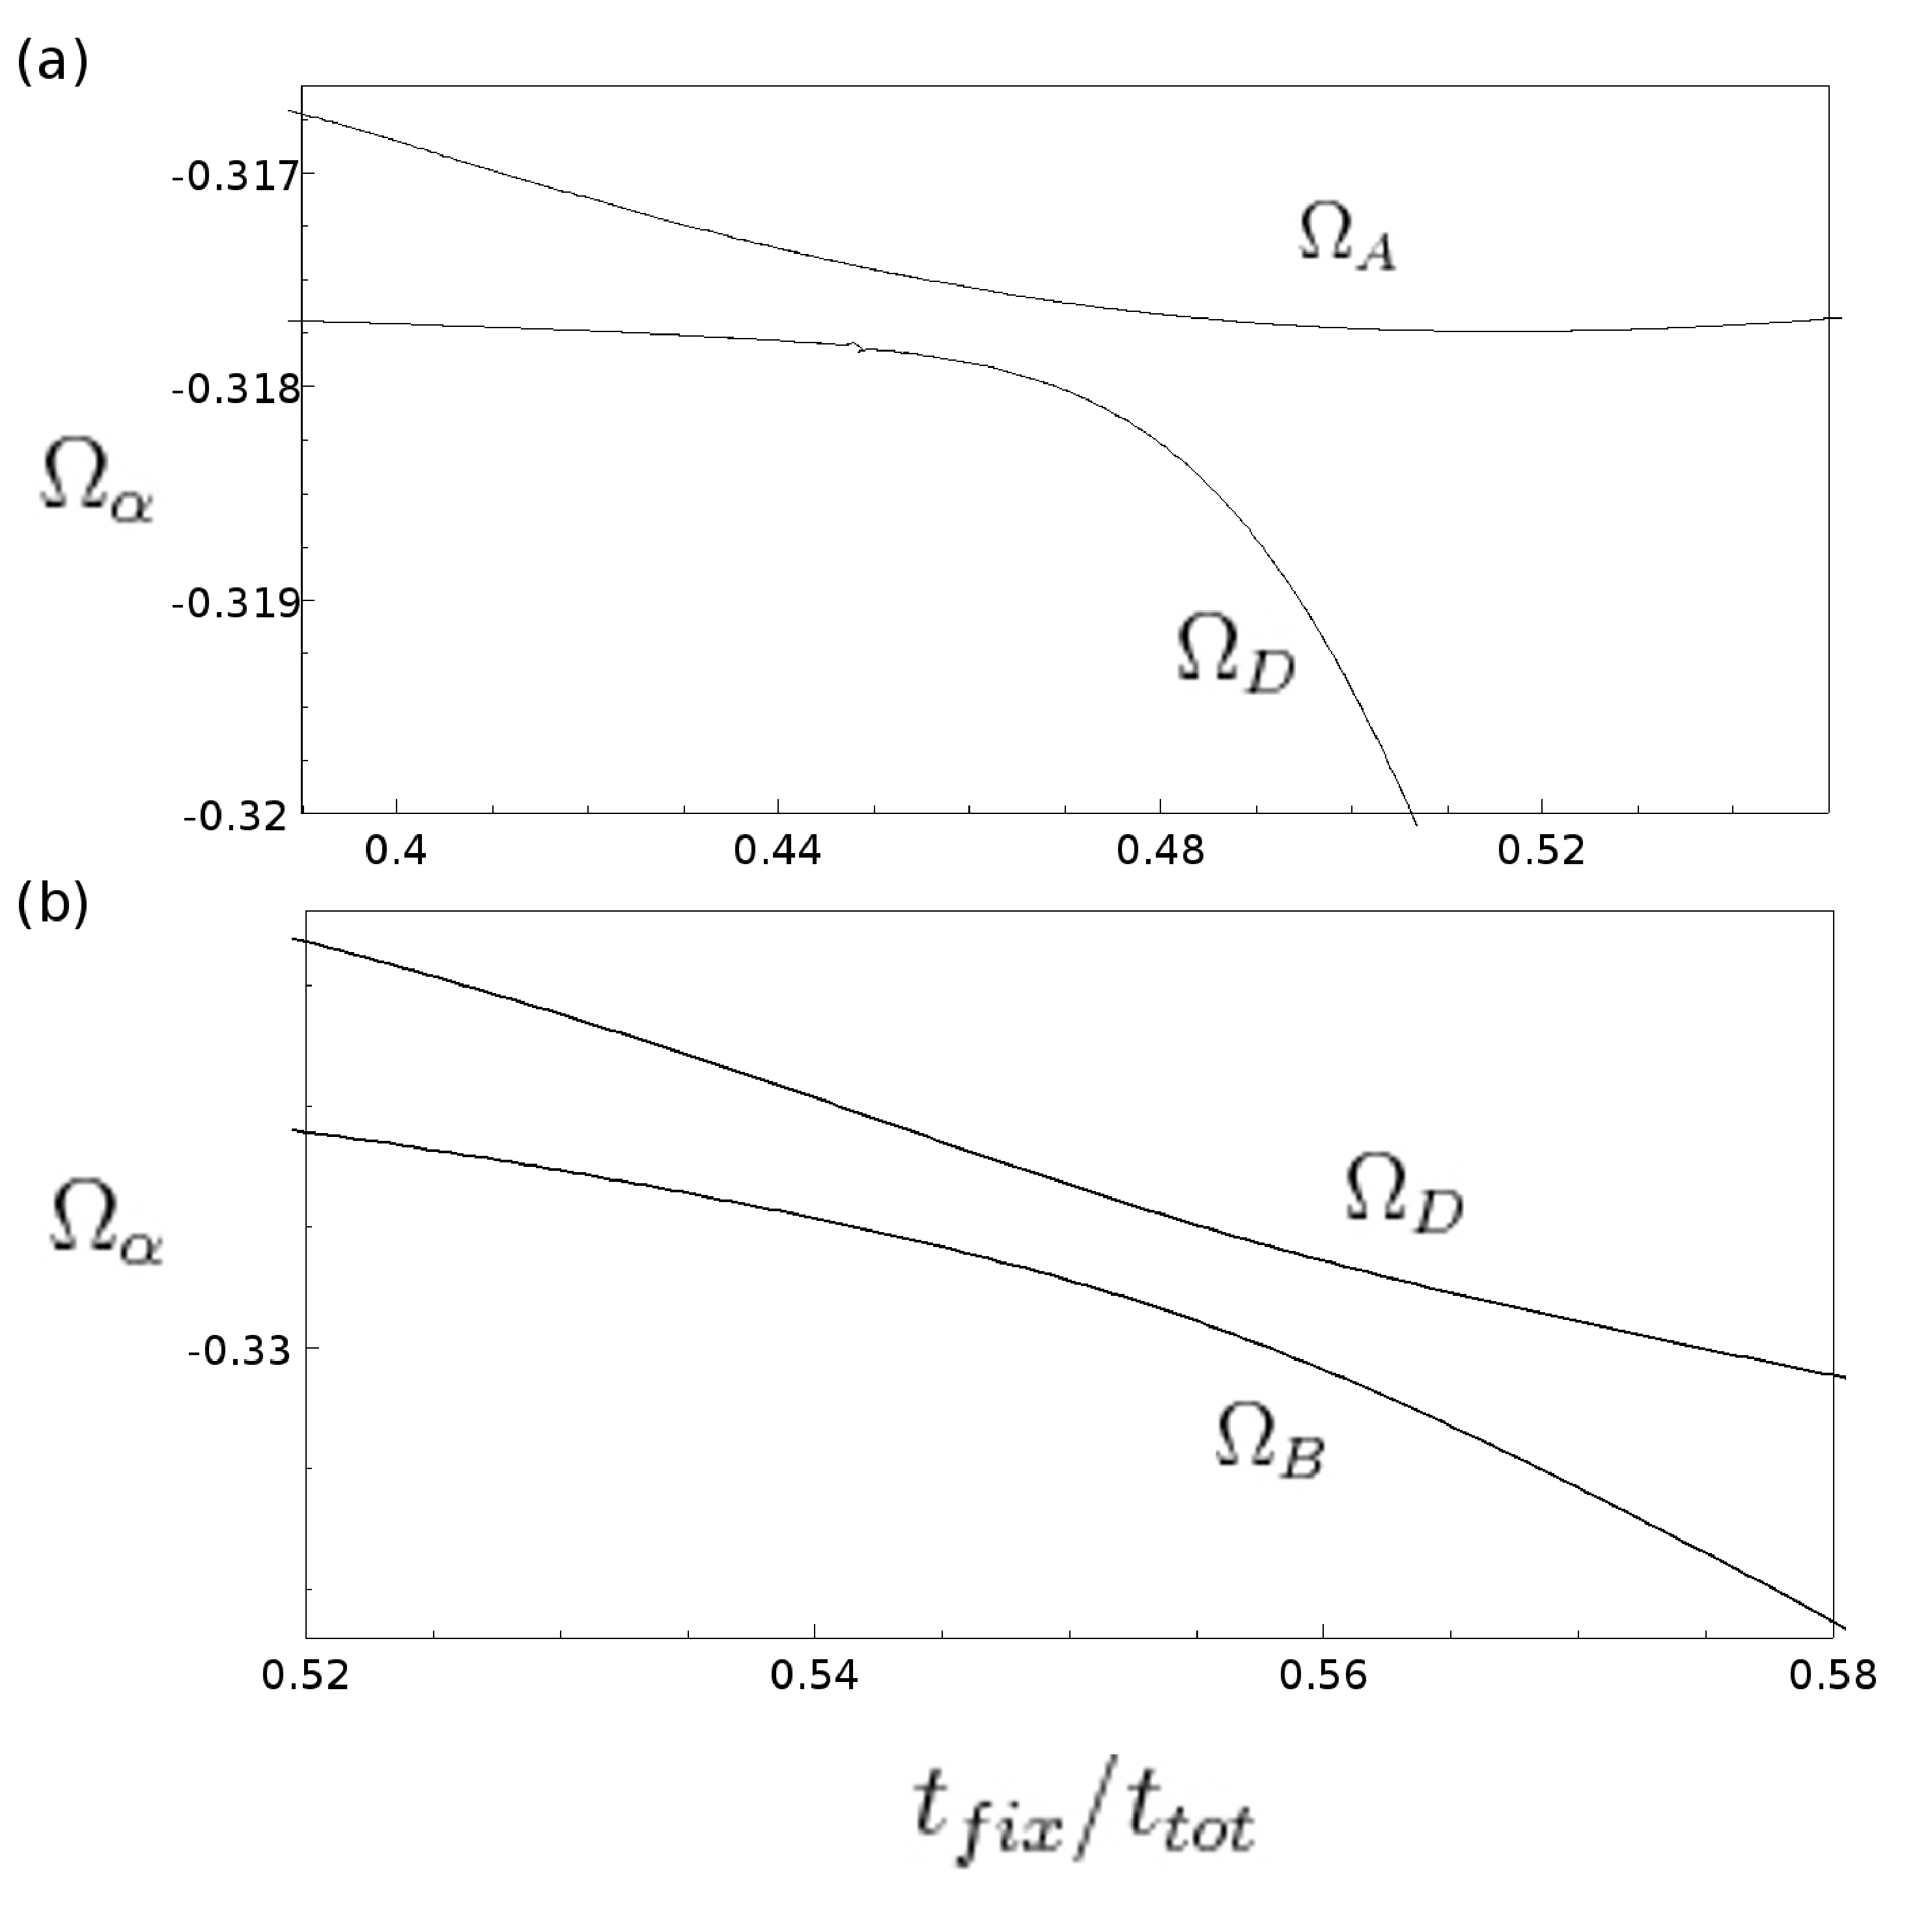
\psfig{file=jpegs/chapter-optical_lattice/fig9.eps,height=6.5in,width=4.5in}
\caption{Magnified views of the $AD$ and $BD$ avoided crossings from the Floquet eigenphase plots in Fig~\ref{fig:floquet_quasi_0.2:chapter-oplattice}. Figure (a) shows the $AD$ crossing and Fig (b) shows the $BD$ crossing. As in Fig~\ref{fig:floquet_quasi_0.2:chapter-oplattice}, the quasienergies $\Omega_\alpha$ are plotted as a function of $t_{fix}/t_{tot}$, where $t_{tot}$ is the total time for the STIRAP pulses.}
\label{fig:floquet_states_0.2:mag:chapter-oplattice}
\end{figure}
